\section{Nondeterministic automata}

A right-linear grammar may contain two alternative rules starting with the same character. 
This means that in state $A$, reading the character, the machine can choose which one of the next states to enter: its behavior is not deterministic. 
A machine move that does not read an input character is termed spontaneous or an epsilon move. 
Spontaneous moves too cause the machine to be nondeterministic. 

The main advantages of having nondeterminism are: 
\begin{itemize}
    \item The correspondence between grammars and automata suggest having:
        \begin{itemize}
            \item Moves with two or more destination states. 
            \item Spontaneous moves (or $\varepsilon$-moves).
            \item And two or more initial states.
        \end{itemize}
    \item Concision: defining a language by means of a non-deterministic automaton may be more readable and compact than using a deterministic one.
\end{itemize}

\subsection*{Nondeterministic finite state automaton}
\begin{definition}
    A \emph{non-deterministic finite automaton} $N$, without spontaneous moves, is defined by: 
    \begin{itemize}
        \item The state set $Q$. 
        \item The terminal alphabet $\Sigma$. 
        \item Two subsets of $Q$: the set $I$ of the initial states and the set $F$ of final states.
        \item The transition relation $\delta$, a subset of the Cartesian product $Q\times\Sigma\times Q$.     
    \end{itemize}
\end{definition} 
A computation of length $n$ originates at state $q_0$ and ends at state $q_n$, and has labeling $a_1a_2\dots a_n$
\begin{definition}
    An input string $x$ is \emph{accepted} by the automaton if it is the labeling of a path that starts from an initial state and ends to a final state: 
    \[L(N)=\{x \in \Sigma^{*}|q \overset{x}{\rightarrow} \textnormal{ with } q \in I \textnormal{ and } r \in F\}\]
\end{definition}
The moves of the non-deterministic automaton can be defined by means of a many-valued transition function. 

For a machine $N=(Q,\Sigma,\delta,I,F)$, without spontaneous moves, the transition function $\delta$ s defined as to have the domain and image: 
\[\delta:Q\times\left(\Sigma\cup\{\varepsilon\}\right)\rightarrow \mathcal{P}(Q)\]
where symbol $\mathcal{P}(Q)$ indicates the power set of set $Q$. 

A non-deterministic automaton may have two or more initial states. 
But it is easy to construct an equivalent non-deterministic automaton with only one initial state. Add a new initial state $q_0$, connect it to the existing initial states by $\varepsilon$-arcs, make such states non-initial and leave only $q_0$. 

\subsection*{Correspondence between automata and grammars}
Consider a strictly right-linear grammar $G=(V,\Sigma,P,S)$ and a nondeterministic automaton $N=(Q,\Sigma,\delta,q_0,F)$ (with a unique initial state).
We have that the following equivalences holds: 
\begin{table}[H]
    \centering
    \begin{tabular}{cc}
    \hline
    \textbf{Right-linear grammar}                            & \textbf{Finite state automaton} \\ \hline
    Nonterminal set $V$                                      & Set of states $Q=V$             \\
    Axiom $S=q_0$                                            & Initial state $q_0=S$           \\
    $p \rightarrow aq$, where $a \in \Sigma$ and $p,q \in V$ & \begin{minipage}{.2\textwidth}\centering
\includegraphics[width=\linewidth, height=9mm]{images/a.png}\end{minipage}                                \\
    $p \rightarrow q$, where $p,q \in V$                     & \begin{minipage}{.2\textwidth}\centering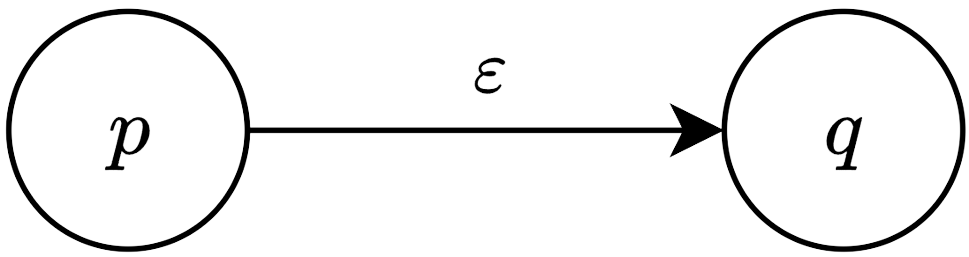
\includegraphics[width=\linewidth, height=9mm]{images/b.png}\end{minipage}                                 \\
    $p \rightarrow a$, where $p,a \in V$ (terminal rule)     & \begin{minipage}{.2\textwidth}\centering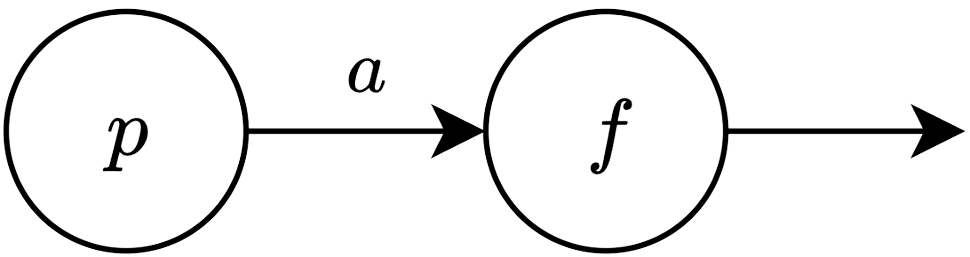
\includegraphics[width=\linewidth, height=9mm]{images/c.png}\end{minipage}                                 \\
    $p \rightarrow \varepsilon$                              & Final state $p$                 \\ \hline
    \end{tabular}
\end{table}
\begin{example}
    Consider the following non-deterministic automaton: 
    \begin{figure}[H]
        \centering
        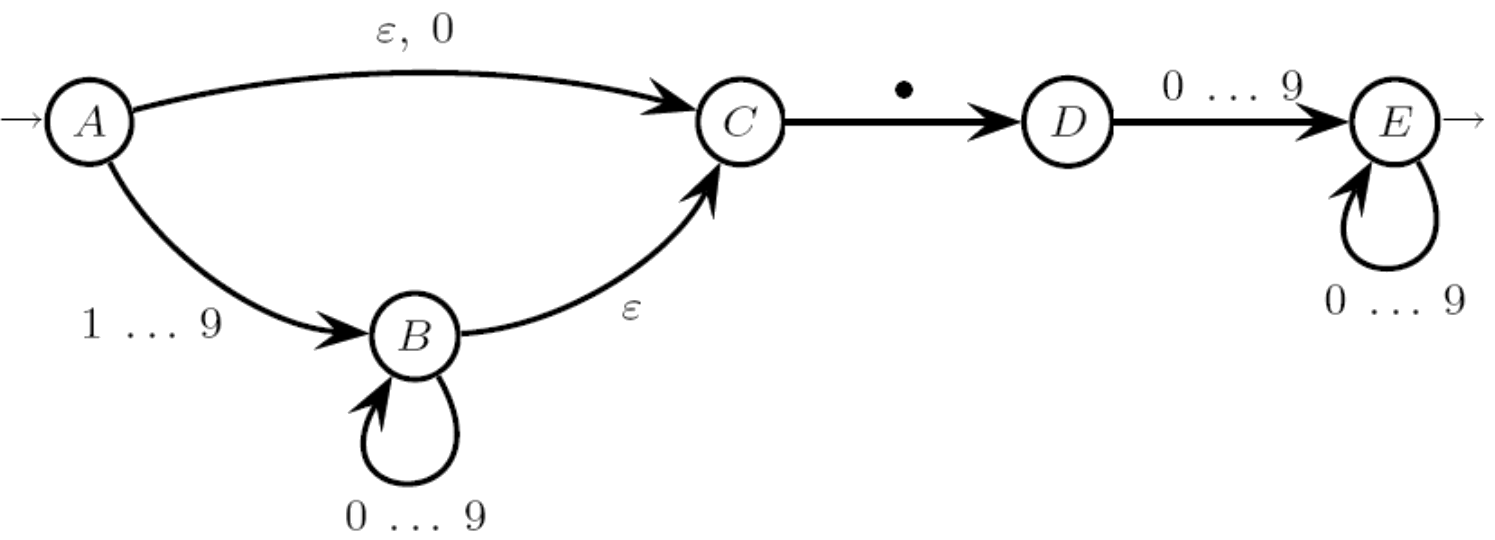
\includegraphics[width=0.5\linewidth]{images/nfsa.png}
    \end{figure}
    It can be easily translated into a grammar following the rules in the table above: 
    \[
    \begin{cases}
        A \rightarrow 0C|C|1B|\dots|9B \\
        B \rightarrow 0B|\dots|9B|C \\
        C \rightarrow \cdot D \\
        D \rightarrow 0E|\dots|9E \\
        E \rightarrow 0E|\dots|9E|\varepsilon

    \end{cases}    
    \]
\end{example}
As a result we have that a grammar derivation corresponds to an automaton computation, and vice versa. 
\begin{proposition}
    A language is generated by a right linear grammar if and only if it is recognized by a finite automaton.
\end{proposition}

\subsection*{Ambiguity}
As grammar derivations are in one-to-one correspondence with automaton computations, ambiguity is extensible to automata.
\begin{definition}
    An automaton is \emph{ambiguous} if, and only if, the corresponding grammar is so, i.e., if a string $x$ labels two or more accepting paths.
\end{definition}
Clearly it follows from the definition that a deterministic automaton is never ambiguous.

REG families can be defined also using left-linear grammars. 
By interchanging left with right, it is simple to discover the mapping between such grammars and automata.